\documentclass[11pt, a4paper, notitlepage]{report}
\usepackage[dvips]{graphicx,color,rotating}
\usepackage{polski}
\usepackage[utf8]{inputenc}
\usepackage{pstricks}
\usepackage{lipsum}
\usepackage{titling}
\usepackage{appendix}
\usepackage{hyperref} 

\pretitle{
	\begin{center} 
		
\includegraphics[width=40pt,height=40pt]{graphics/znak_pk} \\ 
		 \Huge\bfseries}
\posttitle{\par\end{center}\vskip 0.5em}
\preauthor{\begin{center} \Large  KWD  \\  \LARGE\ttfamily}
\postauthor{ \end{center}}
\predate{\par\large\centering}
\postdate{\par}

\pagestyle{headings}

\author{Krzysztof \textsc{Michalski} \\ Rafał \textsc{Pokrywka} }

\title{\textbf{Neuronowy model dawcy krwi}}
\date{27.01.2020}

\pagenumbering{roman} 

\begin{document}
\clearpage\maketitle
\thispagestyle{empty}
\begin{abstract}
	W tym projekcie zajmowaliśmy się przewidywaniem, czy pacjent odda krew w marcu 2007, na podstawie danych z \href{https://archive.ics.uci.edu/ml/datasets/Blood+Transfusion+Service+Center/}{Blood Transfusion Service Center Data Set}. 
	Było to zatem zadanie klasyfikacji binarnej. Zastosowaliśmy kilka modeli - regresję liniową, regresję z użyciem drzew decyzyjnych i lasów losowych oraz w pełni połączoną sieć neuronową. Modele zostały poddane analizie skuteczności i na jej podstawie
	najlepszy okazał się \ldots z dokładnością \ldots 
\end{abstract}

\clearpage \tableofcontents
\thispagestyle{empty}

\setcounter{page}{1}

\chapter{Wprowadzenie}
\pagenumbering{arabic}
	Dane do projektu uzyskaliśmy ze strony \href{https://archive.ics.uci.edu/ml/datasets/Blood+Transfusion+Service+Center/}{Blood Transfusion Service Center Data Set}. Składały się one z dwóch plików {\it transfusion.data} i {\it transfusion.names}.\\ \\
	W pliku  {\it transfusion.data} znajdowało się 748 przykładów opisanych 4 cechami - R (Recency - months since last donation), F (Frequency - total number of donation), M (Monetary - total blood donated in c.c.), T (Time - months since first donation) oraz
	jedną etykietą - binary variable representing whether he/she donated blood in March 2007 (1 stand for donating blood; 0 stands for not donating blood). Zatem zadanie można zaliczyć do kategorii klasyfikacji binarnej. Klasy te były słabo zrównoważone - klasę 1
	posiadało około 24\% przykładów, a klasę 0 - 76\%.\\ \\
	W pliku {\it transfusion.names} znajdował się opis danych - źródło, opis atrybutów oraz autorzy.
\section{Opis problemu}
	Zadanie polega na klasyfikacji binarnej przykładów na podstawie 4 cech numerycznych. Celem klasyfikacji, jest określenie, czy nowy pacjent kliniki odda krew po pewnym okresie czasu. W tym celu można wykorzystać różne techniki uczenia maszynowego 
	takie jak regresja liniowa, drzewa decyzycjne, lasy losowe czy sieci neuronowe. Ze względu na niewielką ilość przykładów oraz cech je opisujących, skuteczność takiej klasyfikacji może być niewielka - zbiory danych o takiej wielkości są niewystarczające 
	dla dobrego wytrenowania na przykład sieci neuronowej. Ze względu na niezrównoważenie klas, modele mogą mieć tendencję do częstszego przewidywania dominującej klasy - bo zapewnia to dużą dokładność takiego modelu. Można spróbować zrównoważyć
	zbiór wybierając podzbiór przykładów o takiej samej reprezentacji klasy pozytywnej i negatywnej.

\chapter{Opis metody}
\section{Wprowadzenie teoretyczne}
\lipsum[1]

\section{Badania symulacyjne}
Analiza zbioru danych w wersji niezrównoważonej:
\begin{verbatim}
+----+-----------+-----------+-----------+------------+------------+
|    |         R |         F |         M |          T |          D |
|----+-----------+-----------+-----------+------------+------------|
| R  |  1        | -0.182745 | -0.182745 |  0.160618  | -0.279869  |
| F  | -0.182745 |  1        |  1        |  0.63494   |  0.218633  |
| M  | -0.182745 |  1        |  1        |  0.63494   |  0.218633  |
| T  |  0.160618 |  0.63494  |  0.63494  |  1         | -0.0358544 |
| D  | -0.279869 |  0.218633 |  0.218633 | -0.0358544 |  1         |
+----+-----------+-----------+-----------+------------+------------+

+-------+-----------+-----------+----------+----------+------------+
|       |         R |         F |        M |        T |          D |
|-------+-----------+-----------+----------+----------+------------|
| count | 748       | 748       |   748    | 748      | 748        |
| mean  |   9.50668 |   5.51471 |  1378.68 |  34.2821 |   0.237968 |
| std   |   8.0954  |   5.83931 |  1459.83 |  24.3767 |   0.426124 |
| min   |   0       |   1       |   250    |   2      |   0        |
| 25%   |   2.75    |   2       |   500    |  16      |   0        |
| 50%   |   7       |   4       |  1000    |  28      |   0        |
| 75%   |  14       |   7       |  1750    |  50      |   0        |
| max   |  74       |  50       | 12500    |  98      |   1        |
+-------+-----------+-----------+----------+----------+------------+
\end{verbatim}

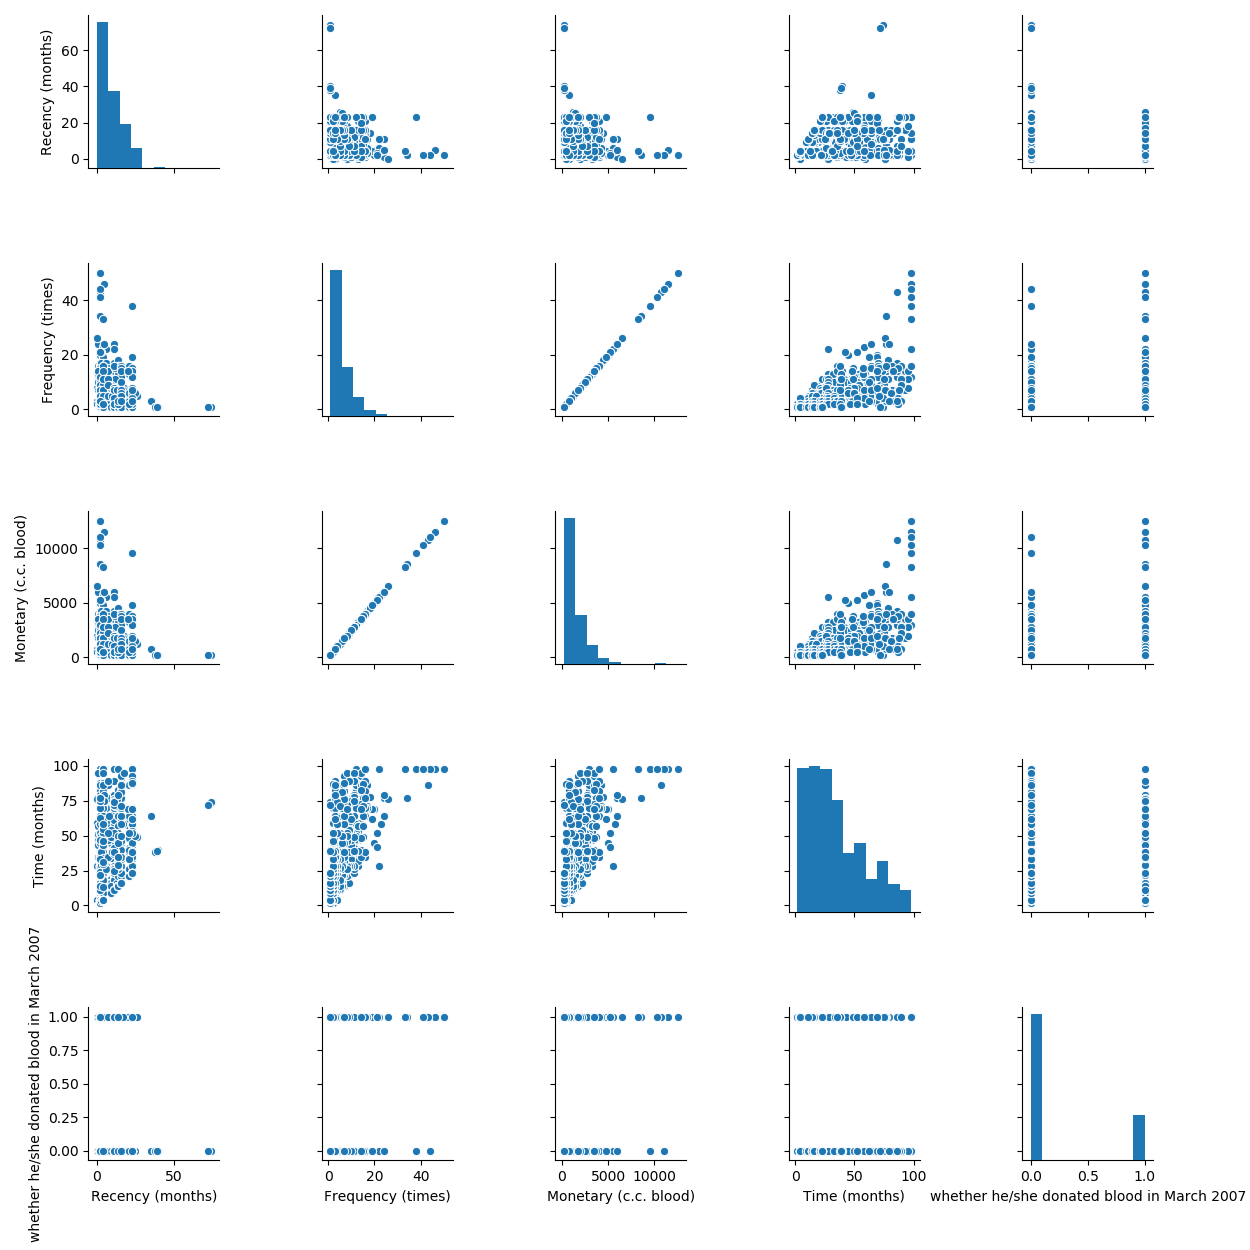
\includegraphics[width=400pt,height=400pt]{graphics/correlation_1} \\ 

Analiza zbioru danych w wersji zrównoważonej:

\begin{verbatim}
+----+------------+-----------+-----------+------------+------------+
|    |          R |         F |         M |          T |          D |
|----+------------+-----------+-----------+------------+------------|
| R  |  1         | -0.218071 | -0.218071 |  0.0949278 | -0.348375  |
| F  | -0.218071  |  1        |  1        |  0.685435  |  0.216987  |
| M  | -0.218071  |  1        |  1        |  0.685435  |  0.216987  |
| T  |  0.0949278 |  0.685435 |  0.685435 |  1         | -0.0152334 |
| D  | -0.348375  |  0.216987 |  0.216987 | -0.0152334 |  1         |
+----+------------+-----------+-----------+------------+------------+

+-------+-----------+-----------+----------+----------+------------+
|       |         R |         F |        M |        T |          D |
|-------+-----------+-----------+----------+----------+------------|
| count | 356       | 356       |   356    | 356      | 356        |
| mean  |   7.95787 |   6.34551 |  1586.38 |  33.0815 |   0.5      |
| std   |   7.19436 |   6.70222 |  1675.55 |  23.8207 |   0.500704 |
| min   |   0       |   1       |   250    |   2      |   0        |
| 25%   |   2       |   2       |   500    |  16      |   0        |
| 50%   |   4       |   5       |  1250    |  28      |   0.5      |
| 75%   |  13.25    |   8       |  2000    |  46      |   1        |
| max   |  40       |  50       | 12500    |  98      |   1        |
+-------+-----------+-----------+----------+----------+------------+
\end{verbatim}

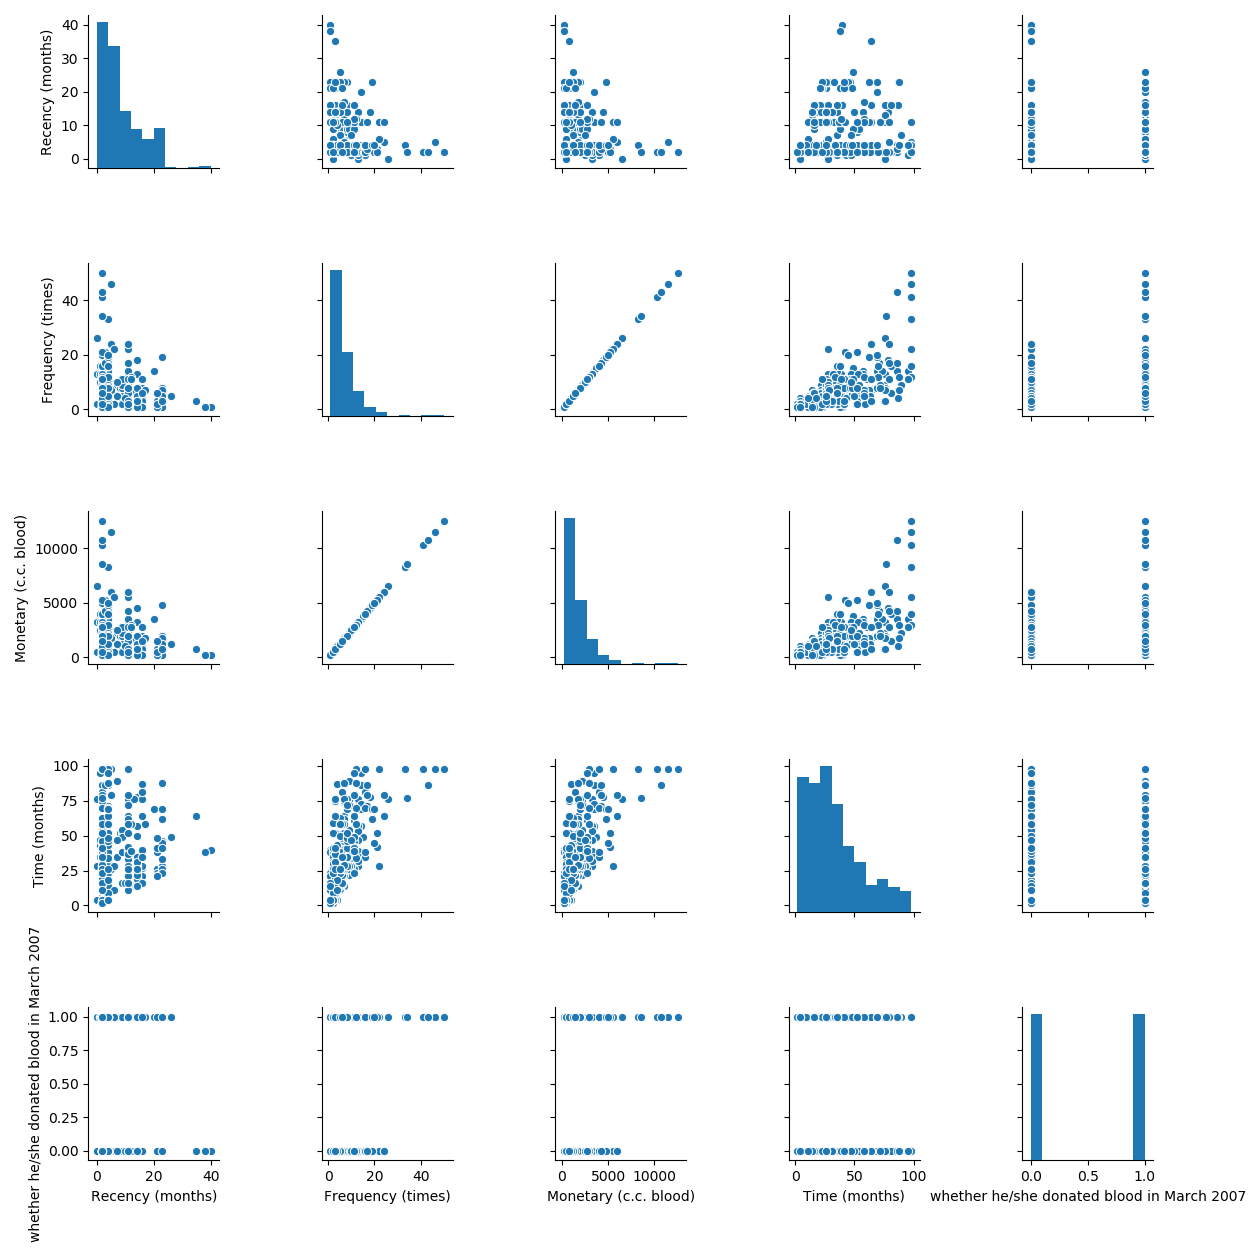
\includegraphics[width=400pt,height=400pt]{graphics/correlation_2} \\ 

\chapter{Podsumowanie}
\lipsum[2]


\begin{appendices}
\chapter{Kod programu}
\begin{verbatim}
import numpy as np

a = np.array([1,2])
b =  np.array([1,2])
c =  a + b
print(c) # printing results
\end{verbatim}
\end{appendices}

\end{document}